\chapter{Optimization}
\label{ch:lesson33}

Chapters~\ref{ch:lesson31}--\ref{ch:lesson32} used plain gradient descent: take the gradient, take a fixed-size step against it, $p\leftarrow p-\eta\nabla f(p)$, where $p$ is whatever's being learned, $\eta$ is the \textbf{learning rate}, and $\nabla f(p)$ is the loss gradient at the current parameters. That's enough to prove the \emph{idea} works, but it's rarely how real networks are trained. This chapter covers four practical upgrades --- \textbf{momentum}, \textbf{adaptive step sizes (Adam)}, \textbf{weight initialization schemes}, and \textbf{learning rate schedules} --- each fixing a specific, concrete failure mode of plain gradient descent.

In real training, the gradient is almost never computed over the \emph{entire} training set at once --- it wouldn't fit into memory. Instead, it's estimated from a small, randomly sampled \textbf{mini-batch} (say, 32 or 256 examples) at every step. The resulting noisy, sample-to-sample-varying estimate is what gives \textbf{stochastic gradient descent (SGD)} its name. This chapter mostly uses the exact, noise-free gradient of a fixed function (calling it ``SGD'' for convenience); the last section simulates mini-batch noise directly to show why it matters.

\section{A loss landscape where plain gradient descent struggles}

$f(x,y)=0.05x^2+5y^2$ is a bowl that's steep in $y$ and shallow in $x$. A step size large enough to make progress along $x$ overshoots along $y$, causing the classic \emph{zigzag}: 30 steps of plain gradient descent leave a final loss of $0.3230$ (Figure~\ref{fig:l33-1}).

\begin{figure}[h]
\centering
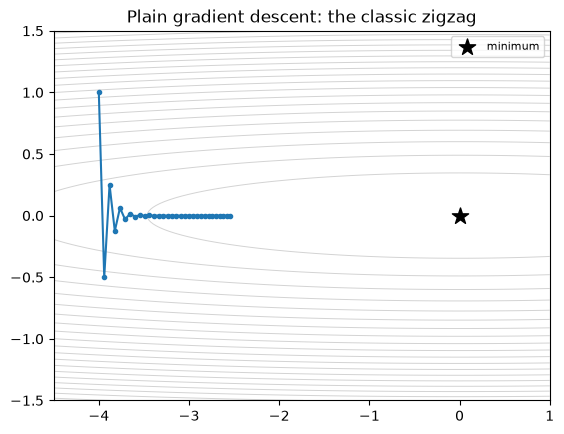
\includegraphics[width=0.55\textwidth]{figures/lesson33_fig01.png}
\caption{Plain gradient descent: the classic zigzag, 30 steps on a narrow bowl.}
\label{fig:l33-1}
\end{figure}

\section{Momentum: remember where you were heading}

Instead of stepping purely along the current gradient, accumulate a running \textbf{velocity} --- a weighted average of past gradients --- and step along that instead:
\begin{equation}
v \leftarrow \beta v - \eta\nabla f(p), \qquad p \leftarrow p + v.
\end{equation}
Momentum's real benefit is acceleration, not damping. Along a consistent direction (the shallow $x$ axis here), every gradient points the same way, so the running velocity keeps growing step after step --- the effective step size along that axis becomes much larger than $\eta$ alone would give, exactly like a ball picking up speed rolling downhill. Along an oscillating direction (the steep $y$ axis, flipping sign every step), consecutive gradients partially cancel in that same running average --- but only \emph{partially}: a single momentum coefficient $\beta$ is shared across every direction, so that cancellation isn't tuned to any one direction's curvature, and the steep axis can still swing substantially before it decays. The net effect, over a full run, is usually still a win: with $\beta=0.9$, 30 steps land at loss $0.2785$ --- better than plain SGD, but by acceleration plus a rough, untuned brake, not a clean fix for oscillation. A from-scratch implementation matches \code{torch.optim.SGD(..., momentum=0.9)} to $2.22\times10^{-16}$.

\section{Adam: per-parameter adaptive step sizes}

\textbf{Adam} (\citelink{kingmaba2014}{Kingma \& Ba, 2014}) tracks both a momentum-like running mean of the gradient ($m$) \emph{and} a running mean of the squared gradient ($v$), then divides the step by $\sqrt{v}$ --- automatically shrinking the step size for parameters with consistently large gradients (like the steep $y$ direction here) and boosting it for parameters with small ones:
\begin{equation}
m \leftarrow \beta_1 m + (1-\beta_1)g, \qquad v \leftarrow \beta_2 v + (1-\beta_2)g^2, \qquad p \leftarrow p - \eta\frac{\hat m}{\sqrt{\hat v}+\epsilon},
\end{equation}
where $\hat m,\hat v$ are bias-corrected versions of $m,v$ (mattering mainly in the first few steps). With $\eta=0.3$ (twice plain SGD's rate), 30 steps reach loss $0.1244$ --- the lowest of the three optimizers, matching \code{torch.optim.Adam} to $1.11\times10^{-16}$.

\begin{figure}[h]
\centering
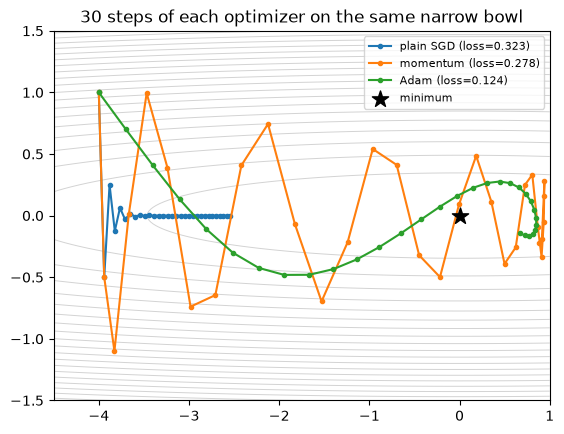
\includegraphics[width=0.6\textwidth]{figures/lesson33_fig02.png}
\caption{30 steps of plain SGD, momentum, and Adam on the same narrow bowl.}
\label{fig:l33-2}
\end{figure}

Figure~\ref{fig:l33-2} makes the difference visible: plain SGD is stuck oscillating across the narrow valley, barely progressing along the shallow direction. Momentum's accumulated velocity clearly accelerates progress along that shallow direction, and it ends with a lower loss than plain SGD --- but notice its path actually swings \emph{wider} in $y$ than plain SGD's own, not narrower, since a single shared momentum coefficient can't damp each axis to the degree that axis specifically needs. Adam, which independently rescales each direction, is what actually tames the steep axis directly, while still racing along the shallow one.

\section{Weight initialization: why zero doesn't work}

It's tempting to initialize all weights to zero. Although this seems like the most ``neutral'' starting point, it's actually catastrophic for any layer with more than one unit: every hidden unit computes the exact same function of the input, gets the exact same gradient, and gets updated by the exact same amount, forever. This \textbf{symmetry} never breaks on its own: training a 4-hidden-unit MLP on the ring-and-disk dataset from zero initialization for 3000 epochs reaches only $50.0\%$ accuracy, with all four hidden units still identical (all zero); randomly initialized weights reach $100.0\%$. Small \emph{random} initialization breaks the symmetry: every unit starts out computing something slightly different, so gradient descent can push them apart and let them specialize. This is why every framework's default layer initialization uses small random values, never zeros.

\section{Weight initialization schemes: how large should ``small random'' be?}

Zero-init fails completely; ``small random'' fixes it. But \emph{how} small? Pick a fixed standard deviation and it works for one layer width, then quietly fails at another. Tracking the variance of activations after passing random data through a deep stack of \code{tanh}-activated linear layers, using a fixed weight std of $0.05$ at every width:

\begin{center}
\renewcommand{\arraystretch}{1.3}
\begin{tabular}{rr}
\hline
\textbf{width} & \textbf{variance after 20 layers} \\
\hline
16  & $7.94\times10^{-28}$ \\
64  & $1.02\times10^{-16}$ \\
256 & $3.12\times10^{-5}$ \\
\hline
\end{tabular}
\end{center}

A fixed std of $0.05$ vanishes to essentially zero after 20 layers --- and the amount it vanishes depends heavily on layer width. Each layer's pre-activation variance scales as $\text{fan\_in}\times\text{std}^2$, where \textbf{fan-in} is the layer's number of inputs: at width 16, that's $16\times0.05^2\approx0.04$, so each layer keeps only about 4\% of the previous layer's variance, and 20 compounding layers erase the signal almost completely. At width 256, the \emph{same} fixed std keeps $256\times0.05^2\approx0.64$ of the variance per layer --- still shrinking, but far more slowly. A fixed std's effect depends entirely on fan-in, so the same number that badly vanishes a narrow layer would, at a wide enough layer, push $\text{fan\_in}\times\text{std}^2$ past 1 and start \emph{exploding} instead.

\textbf{Xavier initialization} (\citelink{glorotbengio2010}{Glorot \& Bengio, 2010}), also known as \emph{Glorot initialization}, fixes this by scaling the std with the layer's fan-in: $\text{std}=\sqrt{1/\text{fan\_in}}$, which keeps $\text{fan\_in}\times\text{std}^2$ pinned at exactly 1 regardless of width. Repeating the experiment with Xavier-scaled weights keeps variance in the same ballpark at every width ($0.026$, $0.023$, $0.027$ at widths 16, 64, 256), instead of vanishing catastrophically --- and \code{nn.init.xavier\_normal\_}'s empirical weight std ($0.0627$) matches the formula's prediction ($0.0625$) closely.

But Xavier's derivation assumes a symmetric activation like \code{tanh}. \textbf{Kaiming initialization} (\citelink{he2015kaiming}{He et al., 2015}), also known as \emph{He initialization}, is the same idea adjusted for \code{ReLU}, which zeros out roughly half its inputs and so needs twice the variance to compensate: $\text{std}=\sqrt{2/\text{fan\_in}}$. Using Xavier's \code{tanh}-derived scale on a \code{ReLU} network still vanishes: at width 256, Xavier scale gives a variance of $3.06\times10^{-7}$ after 20 layers, while Kaiming scale keeps it at $1.324$ --- and \code{nn.init.kaiming\_normal\_}'s empirical std ($0.0887$) again matches the formula ($0.0884$).

Rule of thumb: use Kaiming init for \code{ReLU}-family networks (the default for \code{nn.Conv2d}/\code{nn.Linear} is actually already a variant of this), and Xavier for \code{tanh}/\code{sigmoid}. Both are strictly better than picking a fixed std and hoping. They're derived, not tuned, from a simple requirement: keep activation variance roughly constant from layer to layer, so a network can be made arbitrarily deep without silently losing its signal before training even starts.

\section{Learning rate schedules}

A single fixed learning rate for the whole training run is tempting, but it's often the wrong choice: a rate large enough for fast early progress is usually too large to settle precisely once training nears a minimum. \textbf{Learning rate schedules} change the rate over time. Three common ones, each validated against \code{torch.optim.lr\_scheduler} to within numerical roundoff (Figure~\ref{fig:l33-3}):
\begin{itemize}
  \item \textbf{Step decay}: multiply the rate by a fixed factor every $N$ steps.
  \item \textbf{Cosine annealing}: smoothly decay along a cosine curve from the initial rate down to (near) zero --- the name is borrowed directly from \textbf{simulated annealing}, the classical optimization technique of starting ``hot'' (free to explore, even accepting worse moves) and gradually ``cooling'' toward a fixed solution.
  \item \textbf{Linear warmup}: \emph{ramp up} from zero over the first few steps, before applying the main schedule --- used because early updates, before a model's gradient statistics have stabilized, can be unreliable enough that a large rate from step one causes damage a few steps of gradual ramp-up would have avoided.
\end{itemize}

\begin{figure}[h]
\centering
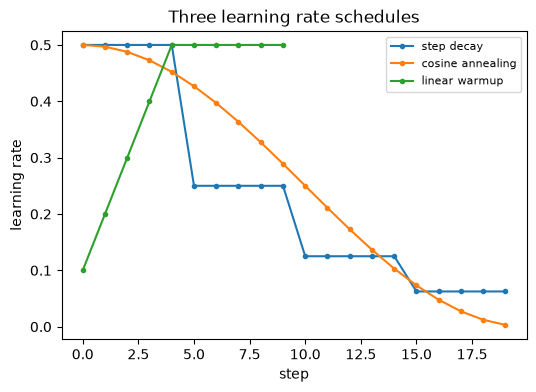
\includegraphics[width=0.6\textwidth]{figures/lesson33_fig03.png}
\caption{Three learning rate schedules: step decay, cosine annealing, and linear warmup.}
\label{fig:l33-3}
\end{figure}

\subsection*{Why decay actually helps: noisy gradients}

On the exact, noise-free narrow bowl from the top of this chapter, a well-chosen constant learning rate converges just fine --- there's nothing to decay away from. Real training almost never sees the exact gradient, though: each step uses a mini-batch estimate, which is noisy. Simulating that by adding random noise to the gradient every step, and comparing a constant rate against step decay: constant learning rate leaves a mean loss over the final 50 steps of $0.2142$, while step decay reaches $0.0025$ --- nearly two orders of magnitude lower (Figure~\ref{fig:l33-4}).

\begin{figure}[h]
\centering
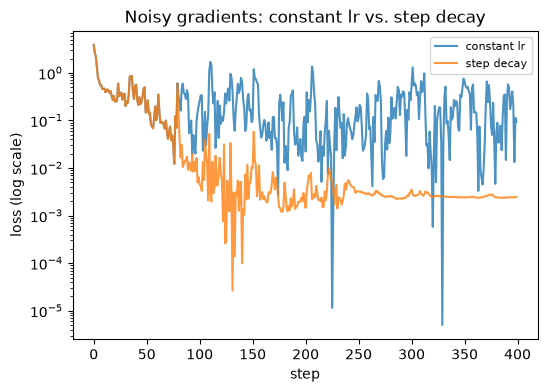
\includegraphics[width=0.6\textwidth]{figures/lesson33_fig04.png}
\caption{Noisy gradients: constant learning rate vs.\ step decay, loss on a log scale.}
\label{fig:l33-4}
\end{figure}

With noisy gradients, a constant learning rate large enough to make fast early progress never actually settles --- it keeps bouncing around the minimum by an amount proportional to the learning rate itself, forever. Step decay makes the same fast early progress, then shrinks the rate as training continues, tightening that bounce and landing far closer to the true minimum. This is the real justification for learning rate schedules: not that a fixed rate is ``wrong'' on some idealized noise-free problem, but that it can't simultaneously be large (for speed) and small (for precision) when every gradient is a noisy estimate, which is the normal situation for real mini-batch training.

\subsection*{Exercises}
\begin{enumerate}
  \item Increase \code{momentum} from 0.9 to 0.99 on the narrow-bowl problem. Does it converge faster, or does it start to overshoot the minimum and oscillate on the \emph{shallow} axis now?
  \item Try initializing the MLP's weights identically but nonzero instead of all-zero. Does symmetry still fail to break?
  \item Adam's learning rate (0.3) is much larger than plain SGD's (0.15), yet Adam remains stable while a plain SGD run at that rate would diverge on the steep axis. Try it and confirm. What does that suggest about why Adam is often described as being more forgiving of the learning-rate choice?
  \item Rerun the Xavier-vs-Kaiming comparison at width 16 and width 1024. Does the gap between the two get bigger or smaller as width grows, matching the fan-in scaling argument used to derive both formulas?
  \item In the noisy-gradient learning-rate demo, try \code{noise\_std=0.0} (no noise at all). Does step decay still help, hurt, or make no difference relative to a constant rate?
\end{enumerate}

\vfill
\fullcode{lesson33}{lesson33_optimization}
